% !Mode:: "TeX:UTF-8"
% !TEX program  = xelatex
\documentclass[a4paper]{article}
\usepackage{amsmath}
\usepackage{amssymb}
\usepackage{ctex}
%\usepackage{braket}
\usepackage[european]{circuitikz}
\usepackage{multirow}
\usepackage{float}
\usepackage{geometry}
\geometry{left=2.5cm,right=2.5cm,bottom=2.5cm,top=2.5cm}
\title{模电实验报告6:有源RC电压放大实验}
\author{xy\quad 学号\quad 匡亚明学院}
\date{2019年2月29日}
\begin{document}
\maketitle
\bibliographystyle{unsrt}
%--------main-body------------

\section{实验目的}
\begin{enumerate}
\item 学习有源RC电压放大器.本实验有三个电路,同相输入放大器,反相输入放大器,三运放仪器放大器.
\end{enumerate}

\section{实验仪器}
示波器、信号发生器、交流毫伏表、数字万用表.

\section{预习内容}
\begin{enumerate}
\item 阅读LF353的“数据手册”,了解LF353的性能.
\item 复习关于用运放和RC组成的电压放大器的理论知识.
\item 阅读本次实验的教材,学习关于计及运放频率特性的有源RC电路的分析方法.
\end{enumerate}

\section{实验原理}
\subsection{运算放大器与有源RC电路}
图(\ref{cd1})是LF353数据手册中给出的简化原理图.由图可见,它可划分为三个单元电路.第一个单元是由漏极电流源$I_1$、场效应管$Q_1$、$Q_2$和源极恒流源负载(由$Q_3$、$D_1$、$R_1$、$R_2$组成)组成的差动放大器.容易看出,它有很高的输入电阻和很大的CMRR(共模抑制比).第二个单元是由集电极电流源$I_2$、第三个单元防输出交越失真二极管$D_2$、$D_3$、三极管$Q_4$和交流电压负反馈电容$C_1$组成.容易看出,它有很高的电压放大倍数.第三个单元是由$Q_5$、$Q_6$和防输出交越失真二极管$D_2$、$D_3$组成的甲乙类功率放大器.容易看出,它放大电流,使运放有一定的带负载能力,亦使运放的输出电阻足够小.通常,集成运放是高输入电阻、高电压放大倍数、低输出电阻的放大器.它由多个功能不同的放大单元电路级连组成.根据级连位置,在图5.1中称第一级差动放大器为输入放大器或前置放大器,称第二级电压放大器为通道放大器,称第三级甲乙类功率放大器为输出放大器.显然,这三个放大单元电路在整个运放中的位置是不能改变的.
\begin{figure}[!h]
\centering
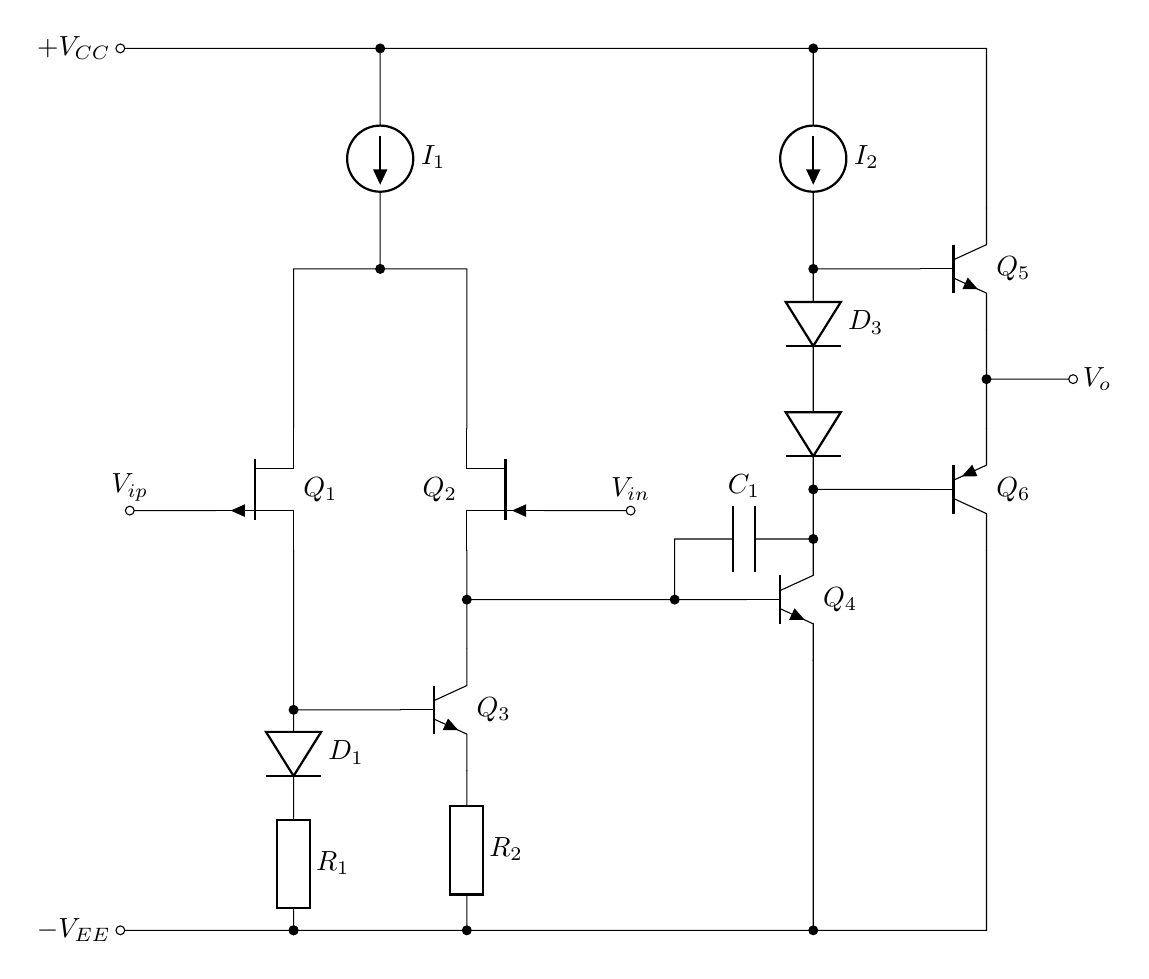
\begin{tikzpicture}[x = 2.2cm, y = 2.8cm]
	\draw[color = black]
	(1,2) node[pjfet, yscale = -1](Q1){} node[anchor = west]{$Q_1$}
	(2,2) node[njfet, xscale = -1](Q2){} node[anchor = east]{$Q_2$}
	(2,1) node[npn](Q3){} node[anchor = west]{$Q_3$}
	(4,1.5) node[npn](Q4){} node[anchor = west]{$Q_4$}
	(5,3) node[npn](Q5){} node[anchor = west]{$Q_5$}
	(5,2) node[pnp](Q6){} node[anchor = west]{$Q_6$}

	(0,0) node[anchor = east]{$-V_{EE}$} to [short, o-*] (1,0)
		  to [short, -*] (2,0)
		  to [short, -*] (4,0) -| (Q6.C)
	(Q6.E) -- (Q5.E)
	(5,2.5) to [short, *-o] (5.5,2.5) node[anchor = west]{$V_o$}
	(Q5.C) |- (0,4) node[ocirc]{} node[anchor = east]{$+V_{CC}$}
	(4,4) to [american current source, *-*, l= $I_2$] (4,3)
		  to [D, l=$D_3$] (4,2.5)
		  to [D, -*] (4,2) -- (Q4.C)
	(4,3) -- (Q5.B)
	(4,2) -- (Q6.B)
	(Q4.C) to [C, l_=$C_1$, *-] ++(-0.8,0)
		   to [short, -*] (3.2,1.5) -- (Q4.B)
	(Q4.E) -- (4,0)
	(3.2,1.5) -| (Q2.S)
	(Q3.C) to [short, -*] (2,1.5)
	(Q3.E) to [R = $R_2$] (2,0)
	(Q3.B) to [short, -*] (1,1)
		   to [D, l=$D_1$] (1,0.6)
		   to [R, l=$R_1$, -*] (1,0)
	(1,1) -- (Q1.S)
	(1.5,4) to [american current source, *-*, l= $I_1$] (1.5,3)
	(1.5,3) -| (Q2.D)
	(1.5,3) -| (Q1.D)
	(Q2.G) to [short, -o] ++(0.5,0) node[anchor = south]{$V_{in}$}
	(Q1.G) to [short, -o] ++(-0.5,0) node[anchor = south]{$V_{ip}$}
	;
\end{tikzpicture}
\caption{LM353等效原理示意图}\label{cd1}
\end{figure}
通常,一个实用的放大器至少也应包括输入放大器、通道放大器和输出放大器.在已做过的四个实验中的放大电路都是放大单元电路,并不是一个实用的放大器.其中,实验1是没有交流负反馈的电压放大器,在实际中很少使用;实验2是有交流负反馈的电压放大器,可用做通道放大器;实验3是差动放大器,若去掉输入端的$R_{b1}$、$R_{b2}$,可用做输入放大器;实验4是甲乙类功率放大器,可用做输出放大器.
\newpage
理想运放有以下假设(并非是理想运放的全部假设):
\begin{enumerate}
\item 开环增益无穷大,$A_{A_0}\to\infty$.
\item 输入阻抗无穷大,$R_{ai}\to\infty$.
\item 共模抑制比无穷大,CMRR$\to\infty$.
\item 输入失调电压为零,$V_{ioff}\to$0.
\item 输入失调电流为零,$I_{ioff}\to$0.
\item 输出电阻为零,$R_{A_o}\to$0.
\end{enumerate}
以上假设使电路分析大大简化,得到的结果往往十分简洁.
实际运放的前三项都不是无穷大,后三项也都不为零.
在实际电路中,电路的实际性能指标与设计值之间有差别这是不可避免的,只要这种差别足够小,或在允许的范围内,就可以认可.例如:
\begin{enumerate}
\item 当运放的开环增益大于大于用运放构成的闭环放大器的闭环增益时,就可以认为运放的开环增益无穷大,即$A_{A_0}\to\infty$.
\item 当运放输入端所接电阻的阻值远小于小于运放输入电阻时,就可以认为运放的输入阻抗无穷大,即$R_{ai}\to\infty$.
\item 当用运放构成的放大器的输入电阻远小于小于共模干扰源内阻时,就可以认为运放共模抑制比无穷大,即CMRR$\to\infty$.
\item 当运放直流闭环后,输入信号电压大于大于输入失调电压时,就可以认为运放的输入失调电压为零,即$V_{ioff}\to0$.
\item 当与运放输入端相连元件中的电流大于大于输入失调电流时,就可以认为运放的输入失调电流为零,即$I_{ioff}\to0$.
\item 当运放输出端所接负载电阻远大于大于运放输出电阻时,就可以认为运放的输出电阻为零,即$R_{A_o}\to0$.
\end{enumerate}
在许多场合,理想运放的假设并不成立.例如:
某运放在10kHz处的开环增益为100,用该运放组成的反向输入放大器,用理想运放假设按闭环增益为20倍设计.当输入信号频率为10kHz时,放大器的实际放大倍数约为16倍.可见,这里就不能假设运放的开环增益为无穷大.
某运放的CMRR为100dB,而要求设计的放大器输入阻抗大于2M$\Omega$,共模抑制比大于93dB,这时候就不能假设运放的CMRR无穷大.
某电压型运放的输出电阻为60$\Omega$,通常要求负载大于等于2k$\Omega$,运放才能正常工作,才能假设运放$R_{A_o}\to0$.若负载电阻过小,例如,负载被误接为100$\Omega$,则运放不能正常工作,还有可能损坏运放.
实验6图(1)所示积分器,由于直流开环,运放直流开环增益很大,运放输入端的直流失调电压将乘以开环放大倍数被放大,往往使输出直流超过运放的直流偏置电压,积分器因阻塞而不能工作.这时就不能假设运放输入失调电压为零.
称由R、C和运放组成的电路为有源RC电路.这是一类广泛使用的电路.用运放和RC的电压放大器是有源RC电路中的一类电路.
在电子专业教学计划中,通常“模拟电路”是第一门电子技术课.在此之前,学习者大都仅仅学习了“电路分析”或/和“电工学”,可能只有少数学校已讲授了“信号与系统”.所以,为了简化,在模拟电路课程中往往以“理想运放”为基础讲述有源RC电路.实际情况是:由“理想运放”导出的对有源RC电路的描述往往在几kHz以上的频段上就与实际电路有差别,甚至有很大差别.电路实验课的内容是面对实际电路的.在以后关于运放的实验中,将主要强调用计及运放频率特性的分析方法分析有源RC电路,由此导出的对有源RC电路的描述与实际电路的差别将大大缩小.
\subsection{运放的频率特性}
运放被认为是线性电路.由线性系统理论,当电路的输入
\begin{equation}
x(t) = X_)\sin(\omega t+\varphi_x)\label{5.1}
\end{equation}
为正弦波时,则输出y(t)为与x(t)同频率的正弦波,其幅值被电路|H(j$\omega$)|加权,相位被延迟$\varphi_H$($\omega$)
\begin{equation}
y(t) = |H(j\omega)|X_0\sin\left(\omega t+\varphi_x+\varphi_H(\omega)\right)\label{5.2}
\end{equation}
称
\begin{equation}
H(j\omega) = \cfrac{Y(j\omega)}{X(j\omega)} = |H(j\omega)|e^{j\varphi_H(\omega)}\label{5.3}
\end{equation}
为电路的频率特性函数,其中,|H(j$\omega$)|为幅频特性函数,$\varphi_H$($\omega$)为相频特性函数.对实际电路,即物理可实现系统,$\varphi_H$($\omega$)$\leq$0.由线性系统理论还可知,对于最小相位线性系统的幅频特性与相频特性不是相互独立的,即已知幅频特性可以导出相频特性,已知相频特性可以导出幅频特性.所以,在后面计及运放的频率特性时,往往仅使用其幅频特性.使用运放的幅频特性与使用运放的相频特性是等价的.
\begin{figure}[!h]
\centering
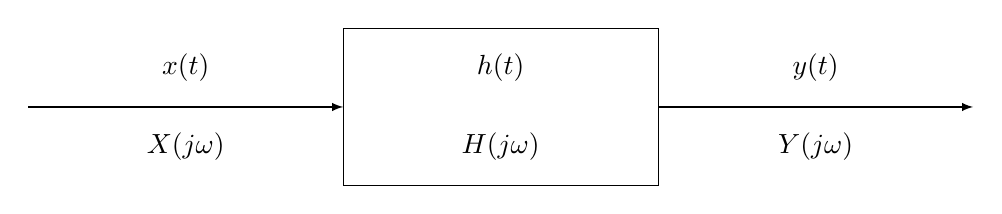
\begin{tikzpicture}[x = 2cm, y = 1cm]
	\draw[color = black]
	(0,0.5) node[]{$h(t)$}
	(0,-0.5) node[]{$H(j\omega)$}
	(-2,0.5) node[]{$x(t)$}
	(-2,-0.5) node[]{$X(j\omega)$}
	(2,0.5) node[]{$y(t)$}
	(2,-0.5) node[]{$Y(j\omega)$}
	(1,1) -- (-1,1) -- (-1,-1) -- (1,-1) -- (1,1);

	\draw[-latex] (-3,0)--(-1,0);
	\draw[-latex] (1,0) -- (3,0);
\end{tikzpicture}
\caption{线性系统的频率特性函数}\label{freqFuncLinSys}
\end{figure}
以OP07为例试述运放的频率特性.由OP07的典型频率特性曲线(又称为Bode图)可知,它是一个典型的二阶系统,其传递函数为
\begin{equation}
A_o = \cfrac{V_o(s)}{V_i(s)} = \cfrac{k_0}{(T_1s+1)(T_2s+1)} = \cfrac{k_0\omega_1\omega_2}{(s+\omega_1)(s+\omega_2)}\label{5.4}
\end{equation}
在稳态
\begin{equation}
A_0(j\omega) = \cfrac{V_o(j\omega)}{V_i(j\omega)} = \cfrac{k_0\omega_1}{(j\omega+\omega_1)(j\omega+\omega_2)}\label{5.5}
\end{equation}
其中,$V_o$(j$\omega$)为运放输出的傅立叶变换,$V_i$(j$\omega$)为运放输入的傅立叶变换.称(\ref{5.5})式为运放的频率特性函数.其中,$k_0$为开环增益,约为112dB,即400000; $f_1$ $\approx$1.5Hz,$\omega$1$\approx$9.425rad/s,$T_1$=1/$\omega$1$\approx$106ms;f2$\approx$270kHz,$\omega$2$\approx$1.696$\times 10^6$rad/s, $T_2$=1/$\omega$2$\approx$589ns;带宽增益积BWG=600kHz.


\section{实验内容}
\subsection{同相输入放大器}
同相输入放大器如图(\ref{cdtxfdq}).
\begin{figure}[!h]
\centering
\begin{tikzpicture}[x = 2cm, y = 2cm]
	\draw[color = black]
	(0,0) node[op amp, yscale = -1](AMP){} node[]{OP-07}
	(AMP.+) to [short, -o] ++(-1,0) node[anchor = south]{$V_i$}
	(AMP.-) to [short, -*] ++(0,-1) node[](A){}
			to [R = $R_1$] ++(0,-1) node[ground]{};
	\draw (A) to [R = $R_2$] ++(1,0) -| (AMP.out) to [short, *-o] ++(1,0) node[anchor = south]{$V_o$};
\end{tikzpicture}
\caption{同相输入放大器}\label{cdtxfdq}
\end{figure}
由电路可立以下方程
\begin{equation}
V_N = \cfrac{R_1}{R_1+R_2}V_o\\
(V_i - V_N)A_o(s) = V_o\label{5.6}
\end{equation}
其中,$A_o$(s)为运放的传递函数.经代数运算可得同相输入放大器的传递函数
\begin{equation}
H(s) = \cfrac{A_o(s)}{1+F\cdot A_o(s)} = \cfrac{A_o(s)}{1+A_o(s)/H(0)}\label{5.7}
\end{equation}
其中,F=$\frac{R_1}{(R_1+R_2)}$为反馈系数;H(0)$\approx$1/F为理想运放假设时的同相输入放大器的电压放大倍数.称0.707$A_o$(0)处的频率为截止频率$\omega_n$.由于$\omega_1 << \omega_2$,所以在以下分析$\omega_n$时将(\ref{5.4})式简化为
\begin{equation}
A_o(s) \approx \cfrac{k_0\omega_1}{s+\omega_1}\label{5.8}
\end{equation}
将(\ref{5.8})式代入(\ref{5.7})式
\begin{equation}
H(s) = \cfrac{k_0\omega_1}{s+\omega_1(1+k_0F)}\label{5.9}
\end{equation}
可见,在计及运放频率特性后,同相输入放大器为一阶低通电路,其截止频率为
\begin{equation}
\omega_n = \omega_1(1+k_0F) = \omega_1(1+k_0\text{H(0)}) \approx \omega_1k_0\text{/H(0)} = \text{BWG/H(0)}\label{5.10}
\end{equation}
若在图(\ref{cdtxfdq})所示电路中,$R_2$=10k$\Omega$,$R_2$=390k$\Omega$,则由(\ref{5.10})式可得
\begin{equation}
f_n \approx 1.5\times 4\times 10^5/40 = 15\text{kHz}\label{5.11}
\end{equation}
可见,理想运放假设时的同相输入放大器的电压放大倍数越大,其通频带越窄.本例的通频带为(0, $f_n$).%图(5)是用EWB仿真的结果.由图可知,其fn约为15.6kHz.可见,使同相输入放大器具有如图5.5所示幅频特性的主要原因是运放的频率特性.

在图(\ref{cdtxfdq})中取$R_1$=10k$\Omega$,$R_2$=390k$\Omega$,运放为OP07,测量同相输入放大器的幅频特性曲线.将运放换为LF353,再测量同相输入放大器的幅频特性曲线.试比较两者的同异,试分析原因.

\subsection{反相输入放大器}
反相输入放大器如图(\ref{cdfxfdq}).
\begin{figure}[!h]
\centering
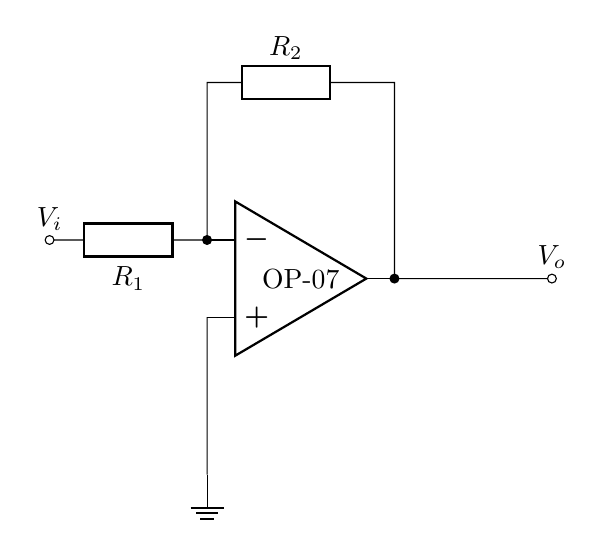
\begin{tikzpicture}[x = 2cm, y = 2cm]
	\draw[color = black]
	(0,0) node[op amp](AMP){} node[]{OP-07}
	(AMP.-) to [R = $R_1$, *-o] ++(-1,0) node[anchor = south]{$V_i$}
	(AMP.-) -- ++(0,1) to [R = $R_2$] ++(1,0) -| (AMP.out) to [short, *-o] ++(1,0) node[anchor = south]{$V_o$}
	(AMP.+) -- ++(0,-1) node[ground]{};
\end{tikzpicture}
\caption{反相输入放大器}\label{cdfxfdq}
\end{figure}
由电路可立以下方程
\begin{equation}
\cfrac{V_i - V_N}{R_1} + \cfrac{V_0 - V_N}{R_2} = 0\\
V_0 = -A_o(s)V_N\label{5.12}
\end{equation}
其中,$A_o$(s)为运放的传递函数.经代数运算可得反相输入放大器的传递函数
\begin{equation}
H(s) = -\cfrac{R_2}{R_1}\cfrac{A_o(s)}{A_o(s)+1+R_2/R_1} = H(0)\cfrac{A_o(s)}{A_o(s)+1-H(0)}\label{5.13}
\end{equation}
其中,H(0)=–$R_2$/$R_1$,为理想运放假设时的反相输入放大器的电压放大倍数.将(\ref{5.8})式代入(\ref{5.13})式
\begin{equation}
H(s) = \cfrac{H(0)}{1-H(0)}\cfrac{k_0\omega_1}{s+\omega_1(1+k_0/(1-H(0)))}\label{5.14}
\end{equation}
可见,在计及运放频率特性后,反相输入放大器亦为一阶低通电路,其截止频率为
\begin{equation}
\omega_n = \omega_1(1+k_0/(1-H(0))) \approx -\omega_1k_0/H(0) = -BWG/H(0)\label{5.15}
\end{equation}
若在图(\ref{cdfxfdq})所示电路中,$R_1$=10k$\Omega$,$R_2$=400k$\Omega$,则由(\ref{5.15})式可得
\begin{equation}
f_n \approx 1.5\times 4\times 10^5/40 = 15kHz\label{5.16}
\end{equation}
可见,在理想运放假设下,反相输入放大器的电压放大倍数越大,其通频带越窄.

在图(\ref{cdfxfdq})中取$R_1$=10k$\Omega$,$R_2$=400k$\Omega$,运放为OP07,测量反相输入放大器的幅频特性曲线.将运放换为LF353,再测量反相输入放大器的幅频特性曲线.试比较两者的同异,试分析原因.

\subsection{有反馈电容的反相输入放大器(一阶低通滤波器)}
电路如图(\ref{1orderfilter}).
\begin{figure}[!h]
\centering
\begin{tikzpicture}[x = 2cm, y = 2cm]
	\draw[color = black]
	(0,0) node[op amp](AMP){} node[]{OP-07}
	(AMP.-) to [R = $R_1$, *-o] ++(-1,0) node[anchor = south]{$V_i$}
	(AMP.-) -- ++(0,1) node[](A){} -- ++(0,1) to [R = $R_2$] ++(1.5,0) -| (1,0) to [short, *-o] ++(1,0) node[anchor = south]{$V_o$}
	(AMP.+) -- ++(0,-1) node[ground]{};
	\draw (A) to [C=$C$, -*] ++(1.59,0)
	(AMP.out) -- (1,0);
\end{tikzpicture}
\caption{一阶低通滤波器}\label{1orderfilter}
\end{figure}
若假设运放开环增益无穷大,则十分容易得到其传递函数,
\begin{equation}
H_1(s) = -\cfrac{R_2}{R_1}\cfrac{1}{R_2Cs+1} = \cfrac{H_0\omega_n}{s+\omega_n} = \cfrac{N_0(s)}{D_0(s)}\label{5.17}
\end{equation}
其中,$H_0$=-$R_2$/$R_1$,$\omega_0$=1/$R_2$C.
计及运放频率特性可立出运放反相输入端电流方程和运放电压传输方程,
\begin{equation}
-V_1g_1+(g_1+g_2+sC)V_N-(g_2+sC)V_o = 0\\
-V_NA_o(s) = V_o\label{5.18}
\end{equation}
其中,g为电导.将上式写成矩阵形式
\begin{equation}
\begin{bmatrix}
g_1+g_2+sC & -(g_2+sC)\\
A_o(s) & 1
\end{bmatrix}
\begin{bmatrix}
V_N\\
V_o
\end{bmatrix}
=
\begin{bmatrix}
V_ig_1 \\
0
\end{bmatrix}
\label{5.19}
\end{equation}
用Cramer法则解方程(\ref{5.19})式可得
\begin{equation}
H_2(s) = \cfrac{H_0\omega_n}{s+\omega_n+\frac{1}{A_o(s)}(s+\omega_0)+\frac{1}{A_o(s)}H_0\omega_n}\\
= \cfrac{N_0(s)}{D_0(s)+D_1(s)+D_2(s)} = \cfrac{N(s)}{D(s)}\label{5.20}
\end{equation}
其中,$N_0$(s)、$D_0$(s)如(\ref{5.17})式,$D_1$(s)=(s+$\omega_n$)/$A_o$(s)=$D_0$(s)/$A_o$(s),$D_2$(s)=$H_0\omega_n$/$A_o$(s)=$N_0$(s)/$A_o$(s).
可见,在计及运放频率特性后,滤波器的传递函数的分母增加了两项$D_1$(s)、$D_2$(s).
在稳态,有s=j$\omega$,因此可有$A_o$(j$\omega$)=$A_o$e$^{j\varphi}$,其中,$A_0$为$\omega$处运放的开环增益,$\varphi$为$\omega$处的相移.对应(\ref{5.20})式绘制矢量图,设$\varphi_0$=-90$^\circ$,如图(\ref{vecAnalyMethod}).由图可知,实际电路由于运放开环增益存在相移$\varphi$,即输出落后于输入,所以整个滤波器的分母矢量增大了,相移也增大了.
\begin{figure}[!h]
\centering
\begin{tikzpicture}[x=2cm,y=2cm]
\draw (0,0) -- (4,0);
\draw (4,0) node[currarrow](x-axis){};
\draw (0,0) -- (0,5) to node[currarrow,rotate=90](y-axis){} (0,5);
\draw (0,0) -- (3,4) to node[currarrow,rotate=50]{} (3,4);
\draw (0,0) -- (2.5,4.5) to node[currarrow,rotate=60]{} (2.5,4.5);
\draw (3,4) -- (2.5,4.2) to node[currarrow,rotate=160]{} (2.5,4.2);
\draw (2.5,4.2) -- (2.5,4.5) to node[currarrow,rotate=90]{} (2.5,4.5);
\draw[dashed] (3,4) -- (0,4);
\draw[dashed] (3,4) -- (3,0);
\draw (-0.2,4) node[]{\LARGE $j\omega$}
	(3,-0.2) node[]{\LARGE $\omega_0$}
	(2.1,2.5) node[]{\LARGE D$_0$}
	(1.5,3) node[]{\LARGE D}
	(3,4.2) node[]{\LARGE D$_1$}
	(2.7,4.5) node[]{\LARGE D$_2$}
	(0.25,5) node[]{\LARGE Im}
	(4,0.25) node[]{\LARGE Re};
\end{tikzpicture}
\caption{矢量分析法}\label{vecAnalyMethod}
\end{figure}
绘制图(\ref{vecAnalyMethod})分析电路的方法称为矢量分析法.它的优点是:对于传递函数分母关于s的代数方程为三阶、四阶时,很难将其做符号因式分解,因此很难从中找到物理意义明确的代数式,并以此分析电路和指导电路设计.对于传递函数分母关于s的代数方程高于五阶时,无代数解.而传递函数分子、分母通常都是以矢量代数和的形式出现,用矢量和的形式可以较容易地清晰地表示传递函数的分子、分母,其物理意义十分显现,可用于分析电路、指导和调整电路设计.

在图(\ref{1orderfilter})中取$R_1$=10k$\Omega$,$R_2$=100k$\Omega$,C=100pF,运放为OP07,测量一阶低通滤波器的幅频特性曲线.将运放换为LF353,再测量一阶低通滤波器的幅频特性曲线.试比较两者的同异,试分析原因.

\subsection{三运放仪器放大器}
三运放仪器放大器电路如图(\ref{3opamp}).
\begin{figure}[!h]
\centering
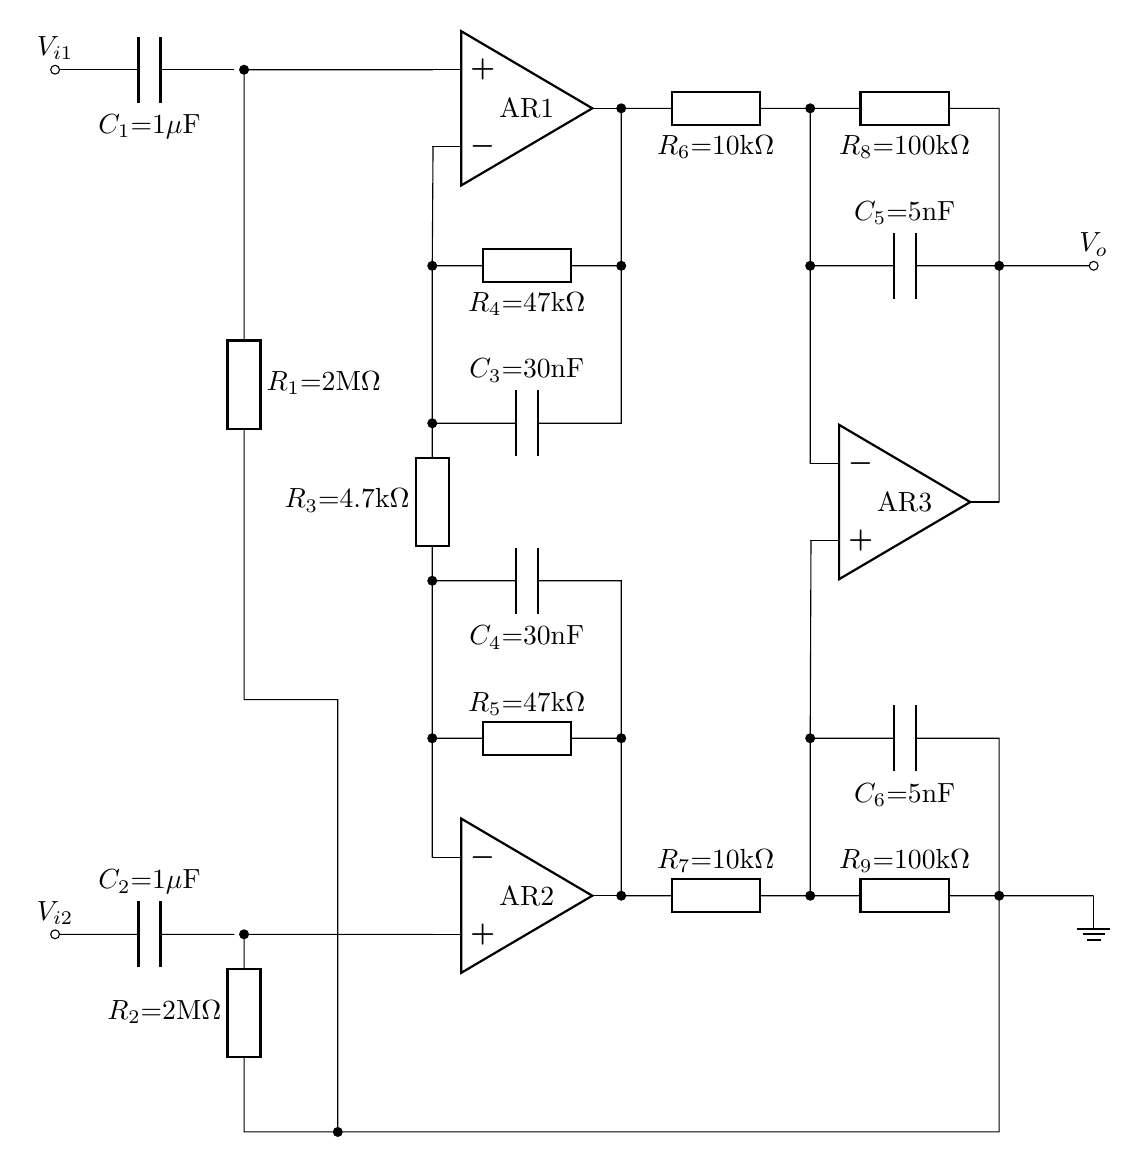
\begin{tikzpicture}[x = 2.4cm, y = 2cm]
	\draw[color = black]

	(0.5,5) node[op amp, yscale = -1](AR1){} node[]{AR1}
	(0.5,0) node[op amp](AR2){} node[]{AR2}
	(2.5,2.5) node[op amp](AR3){} node[]{AR3}

	(AR2.-) -| (0,1)
		to [R = $R_5{=}47\text{k}\Omega$] (1,1) -- (1,2)
		to [C = $C_4{=}30\text{nF}$] (0,2)
		to [R = $R_3{=}4.7\text{k}\Omega$] ++(0,1)
		to [C = $C_3{=}30\text{nF}$] ++(1,0) -- ++(0,1)
		to [R = $R_4{=}47\text{k}\Omega$] ++(-1,0) --(AR1.-)
	(0,1) to [short, *-*] (0,2)
	(0,3) to [short, *-*] (0,4)
	(1,1) to [short, *-*] (1,0)
	(1,4) to [short, *-*] (1,5)

	(1,0) to [R = $R_7{=}10\text{k}\Omega$] ++(1,0)
		  to [R = $R_9{=}100\text{k}\Omega$] ++(1,0) -- ++(0,1)
		  to [C = $C_6{=}5\text{nF}$] ++(-1,0) -- (AR3.+)
	(AR3.-) -| (2,4) to [C = $C_5{=}5\text{nF}$] ++(1,0) -- ++(0,1)
		to [R = $R_8{=}100\text{k}\Omega$] ++(-1,0)
		to [R = $R_6{=}10\text{k}\Omega$] ++(-1,0) -- (AR1.out)
	(2,0) to [short, *-*] ++(0,1)
	(AR3.out) -| (3,4) node[circ]{} to [short, -o] ++(0.5,0) node[anchor = south]{$V_o$}
	(2,4) to [short, *-*] ++(0,1)

	(AR1.+) -- ++(-1,0) node[](A){} to [R = $R_1{=}2\text{M}\Omega$] ++(0,-4) -| (-0.5,-1.5)
	(AR2.+) -- ++(-1,0) node[](B){} to [R, l_= $R_2{=}2\text{M}\Omega$] ++(0,-1) |- (-0.5,-1.5) node[circ]{} -| (3,0) node[circ]{} -- ++(0.5,0) node[ground]{};
	\draw (A) to [C = $C_1{=}1\mu\text{F}$, *-o] ++(-1,0) node[anchor = south]{$V_{i1}$};
	\draw (B) to [C, l_= $C_2{=}1\mu\text{F}$, *-o] ++(-1,0) node[anchor = south]{$V_{i2}$};
\end{tikzpicture}
\caption{三运放仪器放大器}\label{3opamp}
\end{figure}
由于该电路输入电阻大,约为2M$\omega$,通频带约为(0.2Hz, 100Hz),可见该电路容易招来50Hz 共模干扰,所以应使电路具有较大的CMRR,即使电路的共模放大倍数尽可能小.将R9改为91k$\Omega$固定电阻与20k$\omega$可变电阻的串联,用于调整,使电路的共模电压放大倍数尽可能小.在绪论中已做说明,为了使电路的共模电压放大倍数尽可能小,输入端的电容$C_1$、$C_2$和电阻$R_1$、$R_2$应尽可能一致.那么电路中的其它R、C元件与电路共模电压放大倍数有什么关系呢?试分析如下.

为简化分析,将图(\ref{3opamp})简化为图(\ref{3opamp_simplified}).
\begin{figure}[!h]
\centering
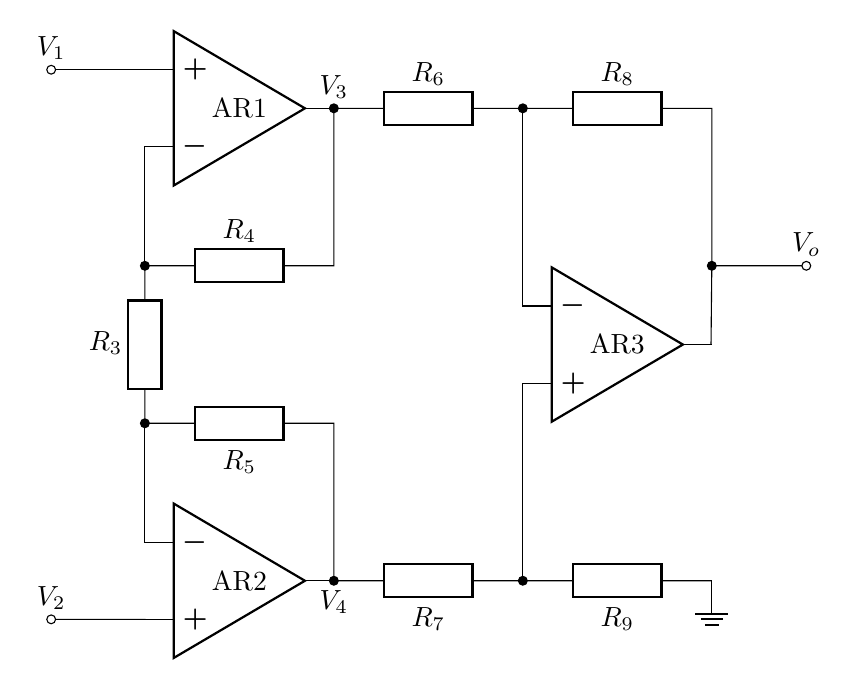
\begin{tikzpicture}[x = 2.4cm, y = 2cm]
	\draw[color = black]

	(0.5,3) node[op amp, yscale = -1](AR1){} node[]{AR1}
	(0.5,0) node[op amp](AR2){} node[]{AR2}
	(2.5,1.5) node[op amp](AR3){} node[]{AR3}

	(3,0) node[ground]{} to [R = $R_9$] ++(-1,0) node[circ](N1){}
		to [R = $R_7$] ++(-1,0) node[anchor = north]{$V_4$} node[](N2){}
		-- ++(0,1)
		to [R = $R_5$] ++(-1,0) node[circ](N3){}
		to [R = $R_3$] ++(0,1) node[circ](N4){}
		to [R = $R_4$] ++(1,0)
		-- ++(0,1) node[anchor = south]{$V_3$} node[circ](N5){}
		to [R = $R_6$] ++(1,0) node[circ](N6){}
		to [R = $R_8$] ++(1,0)
		-- ++(0,-1) node[circ](N7){}
		to [short, -o] ++(0.5,0) node[anchor = south]{$V_o$};

	\draw (N1) |- (AR3.+);
	\draw (N2) to [short, *-] (AR2.out);
	\draw (N3) |- (AR2.-);
	\draw (N4) |- (AR1.-);
	\draw (N5) |- (AR1.out);
	\draw (N6) |- (AR3.-);
	\draw (N7) -- (AR3.out);
	\draw (AR1.+) to [short, -o] ++(-0.5,0) node[anchor = south]{$V_1$};
	\draw (AR2.+) to [short, -o] ++(-0.5,0) node[anchor = south]{$V_2$};
\end{tikzpicture}
\caption{简化的三运放仪器放大器模型}\label{3opamp_simplified}
\end{figure}
为推导共模电压放大倍数,在图中不再假设$R_4$=$R_5$、$R_6$=$R_7$、$R_8$=$R_9$,本例的差模放大倍数约为200倍,通频带约为(0.2Hz, 100Hz),所以可认为运放是近似的理想运放.简化后的三运放仪器放大器共模电压放大倍数推导如下.
当$V_1\neq$0、V2接地($V_2$=0)时,如图(\ref{3opamp_simplified}),对于AR1,AR2输入端“虚短”,AR1、$R_3$、$R_4$等效为同相输入放大器,所以
\begin{equation}
V_3 = (1+\cfrac{R_4}{R_3})V_1\label{5.21}
\end{equation}
对于AR2,AR1输入端“虚短”,$V_{\text{NAR1}}\approx V_1$,$V_{\text{NAR1}}$为AR1反相输入端电压,AR2、$R_3$、$R_5$等效为反相输入放大器,所以
\begin{equation}
V_4 = -\cfrac{R_5}{R_3}V_1\label{5.22}
\end{equation}
利用线性系统的可迭加性,可知由$V_1$引起的输出为
\begin{equation}
V_{o1} = (-\cfrac{R_8}{R_6})(1+\cfrac{R_4}{R_3})V_1+\cfrac{R_9}{R_7+R_9}\cfrac{R_6+R_8}{R_6}(-\cfrac{R_5}{R_3})V_1\label{5.23}
\end{equation}
同理可得当$V_1$=0、$V_2\neq$0时,由$V_2$引起的输出为
\begin{equation}
V_{o2} = \cfrac{R_8}{R_6}\cfrac{R_4}{R_3}V_2+\cfrac{R_9}{R_7+R_9}\cfrac{R_6+R_8}{R_6}(1+\cfrac{R_5}{R_3})V_2\label{5.24}
\end{equation}
当电路的输入为共模电压时,有$V_1=V_2=V_C$,其中$V_C$为共模电压,输出为
\begin{equation}
V_o = V_{o1}+V_{o2} = \cfrac{R_6R_9 - R_7R_8}R_6(R_7+R_9){}V_C\label{5.25}
\end{equation}
共模电压放大倍数为
\begin{equation}
A_{VC} = \cfrac{V_o}{V_C} = \cfrac{R_6R_9-R_7R_8}{R_6(R_7+R_9)}\label{5.26}
\end{equation}
可见,共模电压放大倍数仅与$R_6$、$R_7$、$R_8$、$R_9$有关.若$R_6R_9=R_7R_8$,则共模电压放大倍数为零.
那么是否有可能将$A_{VC}$调得十分接近零呢?做以下共模电压放大倍数的灵敏度分析可知,这是十分困难的.定义电路参数的相对变化率与电路元件值的相对变化率之比为电路参数的灵敏度.例如,对于本例,共模电压放大倍数$A_{VC}$关于电阻$R_6$的灵敏度为
\begin{equation}
S_{R_6}^{A_{VC}} = \cfrac{\text{d}A_{VC}/A_{VC}}{\text{d}R_6/R_6} = \cfrac{R_6}{A_{VC}}\cfrac{\text{d}A_{VC}}{\text{d}R_6} = \cfrac{R_7R_8}{R_6R_9 - R_7R_8}\label{5.27}
\end{equation}
同样,有
\begin{equation}
S_{R_7}^{A_{VC}} = \cfrac{\text{d}A_{VC}/A_{VC}}{\text{d}R_7/R_7} = \cfrac{R_7}{A_{VC}}\cfrac{\text{d}A_{VC}}{\text{d}R_7} = -\cfrac{R_7R_9}{R_6R_9 - R_7R_8}\cfrac{R_6+R_8}{R_6+R_9}\label{5.28}
\end{equation}
因为在设计中要求$R_6$=$R_7$、$R_8$=$R_9$,在实际电路中有$R_6\approx R_7$、$R_8\approx R_9$,所以
\begin{equation}
S_{R_7}^{A_{VC}} = \cfrac{\text{d}A_{VC}/A_{VC}}{\text{d}R_7/R_7} = \cfrac{R_7}{A_{VC}}\cfrac{\text{d}A_{VC}}{\text{d}R_7} \approx -\cfrac{R_7R_9}{R_6R_9 - R_7R_8}\label{5.29}
\end{equation}
同理有
\begin{equation}
S_{R_8}^{A_{VC}} = \cfrac{\text{d}A_{VC}/A_{VC}}{\text{d}R_8/R_8} = \cfrac{R_8}{A_{VC}}\cfrac{\text{d}A_{VC}}{\text{d}R_8} \approx -\cfrac{R_7R_8}{R_6R_9 - R_7R_8}\label{5.30}
\end{equation}
\begin{equation}
S_{R_9}^{A_{VC}} = \cfrac{\text{d}A_{VC}/A_{VC}}{\text{d}R_9/R_9} = \cfrac{R_9}{A_{VC}}\cfrac{\text{d}A_{VC}}{\text{d}R_9} \approx -\cfrac{R_7R_9}{R_6R_9 - R_7R_8}\label{5.31}
\end{equation}
这说明,当$R_6R_9\to R_7R_8$时,共模电压放大倍数的灵敏度将趋向无穷大,实际电路中$R_6$和$R_7$ 、$R_8$和$R_9$不可能完全相等,当$R_6R_9\to R_7R_8$时,$R_6$和$R_7$、$R_8$和$R_9$之间微小差异,将使共模电压放大倍数$A_{VC}$发生较大的变化,所以,实际电路的$A_{VC}$不会等于零.
上述分析还说明,若用一个可变电阻,通过调整可变电阻使实际电路的$A_{VC}$尽可能小,则可用可变电阻替代$R_6$、$R_7$、$R_8$和$R_9$中的任一电阻.本实验电路建议用可变电阻替代$R_9$.
在用可变电阻替代$R_9$后,对于图(\ref{3opamp})所示的电路,要使$A_{VC}$尽可能小,就应使$C_1$与$C_2$、$C_3$与$C_4$、$C_5$与$C_6$、$R_1$与$R_2$、$R_6$与$R_7$尽可能相等.
在面包板上实现图(\ref{3opamp})所示电路,使其$A_{VC}$尽可能小.测量其幅频特性、共模抑制比CMRR、输入端短路时的输入端等效输入噪声电压有效值和等效输入直流漂移.

\section{实验数据}
\subsection{同相放大器}
\begin{enumerate}
\item 波形图\\
同相放大器的波形图如图(\ref{fig1}):
\begin{figure}[!h]
\centering
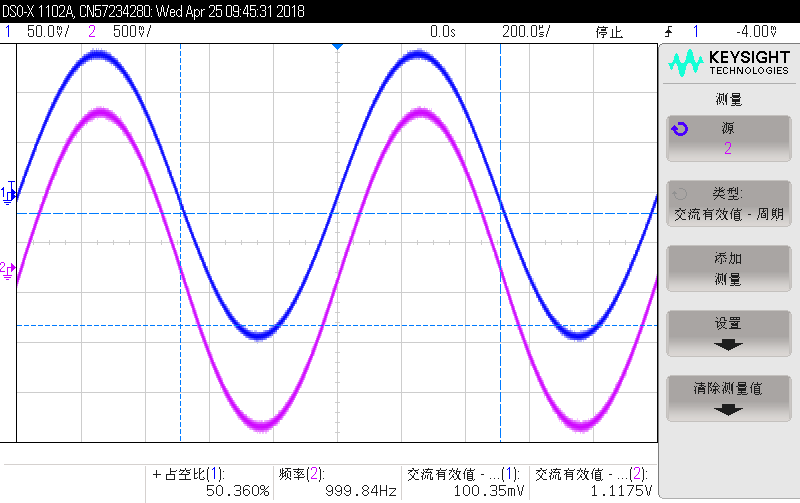
\includegraphics[width=9cm]{fig/1cope_2_r.png}\\
\caption{同相放大器波形图}\label{fig1}
\end{figure}
\item 放大倍数\\
取$R_1$=10k$\Omega$,$R_2$=100k$\Omega$. 测得输入输出电压分别为:\\
$v_i$ = 100.35mV,$v_o$ = 1.1175V.\\
计算得到同相放大器放大倍数为
\begin{equation}
A_V = \cfrac{v_o}{v_i} \approx 11.136
\end{equation}
\item 通频带\\
测量同相放大器的通频带。取中频为1kHz,测得此时输出电压为$v_o$=1.1175V,因此$v_o' = \frac{v_o}{\sqrt{2}} \approx$0.7902V。\\
测得其高频截止频率为:
$$f_H = 38.2\text{kHz}$$
其低频截止频率几乎无法测出。测量高频截止频率时的波形图如图(\ref{fig2}):
\begin{figure}[!h]
\centering
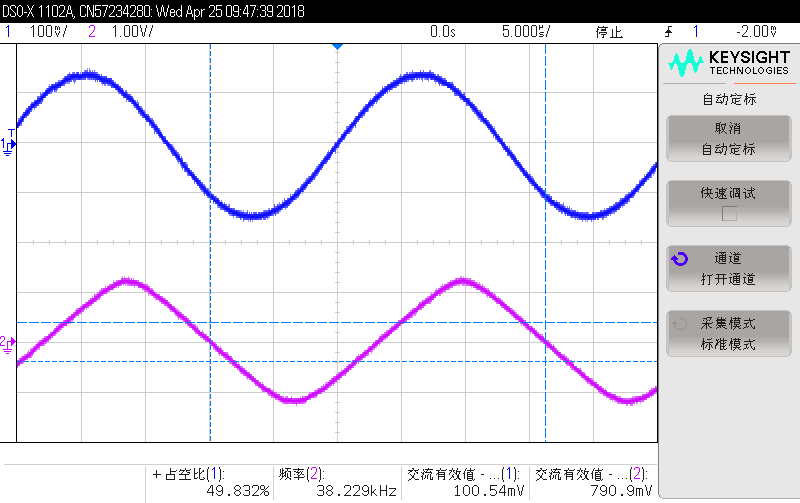
\includegraphics[width=9cm]{fig/2cope_3_r.png}\\
\caption{同相放大器高频截止频率波形图}\label{fig2}
\end{figure}
\end{enumerate}

\subsection{反相放大器}
\begin{enumerate}
\item 波形图\\
反相放大器的波形图如图(\ref{fig3}):
\begin{figure}[!h]
\centering
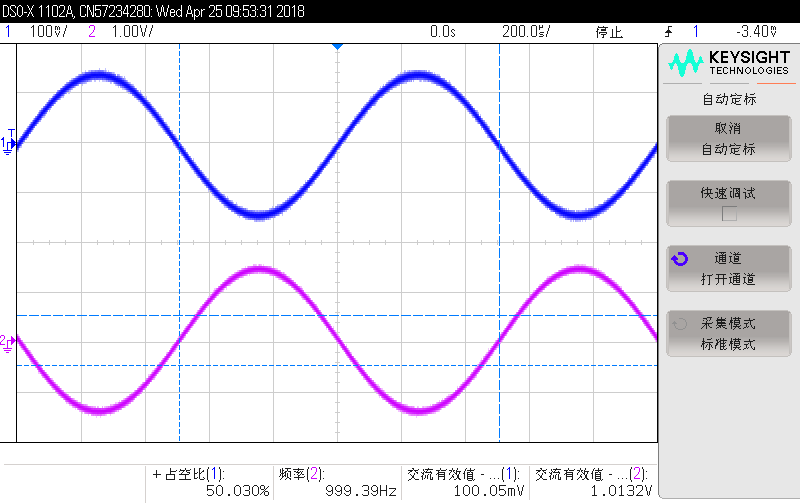
\includegraphics[width=9cm]{fig/3cope_6_r.png}\\
\caption{反相放大器波形图}\label{fig3}
\end{figure}
\item 放大倍数\\
取$R_1$=10k$\Omega$,$R_2$=100k$\Omega$。测得输入输出电压分别为:\\
$v_i$ = 100.05mV,$v_o$ = 1.0132V.\\
计算得到反相放大器放大倍数为:
\begin{equation}
A_V = \cfrac{v_o}{v_i} \approx 10.1269
\end{equation}
\item 通频带\\
测量反相放大器的通频带。取中频为1kHz,测得此时的输出电压为$v_o$=1.0132V,因此$v_o' = \frac{v_o}{\sqrt{2}} \approx 0.7164V$\\
测得其高频截止频率为:
$$f_H = 41.46\text{kHz}$$
其低频截止频率几乎无法测出。测量高频截止频率时的波形图如图(\ref{fig4}):
\begin{figure}[!h]
\centering
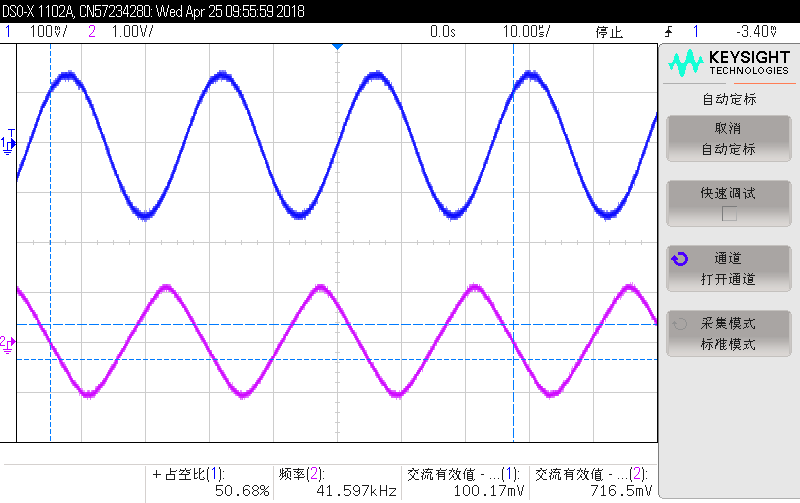
\includegraphics[width=9cm]{fig/4cope_7_r.png}\\
\caption{反相放大器高频截止频率波形图}\label{fig4}
\end{figure}
\end{enumerate}
\subsection{一阶低通滤波器(测通频带)}
\begin{enumerate}
\item C = 100nF\\
取电容$C$ = 100nF时的幅频特性数据如表(\ref{AFC1}):
\begin{table}[!h]
\centering
\caption{低通滤波器幅频特性(C=100nF)}
\label{AFC1}
\begin{tabular}{|c|c|c|c|c|c|c|c|c|c|c|c|}
\hline
f/Hz & 10 & 100 & 200 & 300 & 400 & 500 & 600 & 700 & 800 & 900 & 1000\\ \hline
$v_o$/mV & 840.2 & 150.54 & 76.26 & 51.0 & 38.29 & 30.66 & 25.60 & 22.0 & 19.3 & 17.22 & 15.54\\ \hline
\end{tabular}
\end{table}
\item C = 10$\mu$F\\
取电容$C$ = 10$\mu$F时的幅频特性数据如表(\ref{AFC2}):
\begin{table}[!h]
\centering
\caption{低通滤波器幅频特性(C=10$\mu$F)}
\label{AFC2}
\begin{tabular}{|c|c|c|c|c|c|c|c|c|c|c|}
\hline
f/mHz & 100 & 200 & 300 & 400 & 500 & 600 & 700 & 800 & 900 & 1000\\ \hline
$v_o$/mV & 826.2 & 593.3 & 441.5 & 346.5 & 283.9 & 239.7 & 207.0 & 182.2 & 163.1 & 147.79\\ \hline
f/Hz & 2 & 3 & 4 & 5 & 6 & 7 & 8 & 9 & 10 & \\ \hline
$v_o$/mV & 74.81 & 50.01 & 37.58 & 30.354 & 25.365 & 21.803 & 19.101 & 17.001 & 15.327 & \\ \hline
\end{tabular}
\end{table}
\end{enumerate}
画出不同电容值测得的幅频特性曲线,如图(\ref{AFC_lin}):
\begin{figure}[!h]
\centering
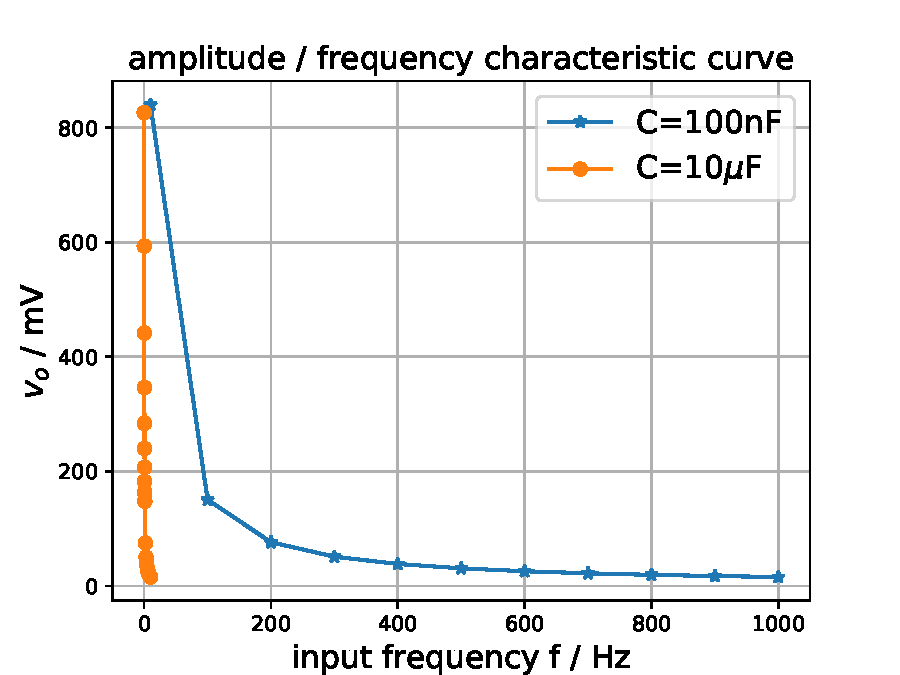
\includegraphics[width=14cm]{fig/AFC_lin.pdf}\\
\caption{幅频特性曲线}\label{AFC_lin}
\end{figure}

可见使用了大电容后的放大器通频带急剧缩窄,已经无法看清高频截止频率,因此我们使用对数坐标重新绘制,如图(\ref{AFC_log}):
\begin{figure}[!h]
\centering
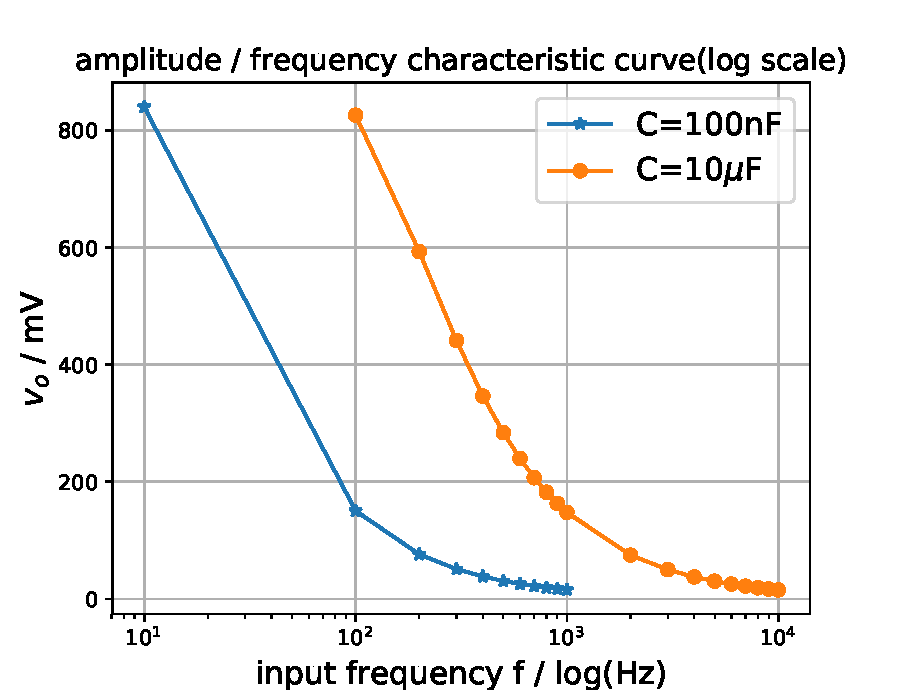
\includegraphics[width=14cm]{fig/AFC_log.pdf}\\
\caption{幅频特性曲线(对数坐标)}\label{AFC_log}
\end{figure}

\section{实验讨论和误差分析}
\begin{enumerate}
\item 低频截止频率\\
在测量同相放大器、反相放大器的通频带时,我们发现几乎无法测出它们的低频截止频率,可知,同相放大器金和反相放大器都几乎可以做直流放大。并且使用示波器读数时发现其示数跳动十分剧烈。
\item 改变电容对低通滤波器的影响\\
由图(\ref{AFC_lin})看出增大电容后,放大器的通频带急剧缩窄,我们读数所取得数据点得分布较为稀疏且在变化较大的地方取点较少,因此可能对画图产生一定影响。
\end{enumerate}

\section{思考题}
\begin{enumerate}
\item \textbf{选同相输入放大器做通道放大器,是否适当?为什么?}\\
不合适,因为会使输入阻抗增大,使信噪比降低。
\item \textbf{若信号源为高内阻信号源,选反相输入放大器做前置放大器,是否适当?为什么?}\\
高内阻信号源不能选反相输入放大器做前置放大器,因为放大倍数会降低。
\end{enumerate}

\nocite{jiaocai}
%--------bib------------------
\bibliography{ref}
\end{document}